\documentclass[a4paper,11pt]{article}
\usepackage{amsmath,amsthm,amsfonts,amssymb,amscd,amstext,vmargin,graphics,graphicx,tabularx,multicol} 
\usepackage[francais]{babel}
\usepackage[utf8]{inputenc}  
\usepackage[T1]{fontenc} 
\usepackage{pstricks-add,tikz,tkz-tab,variations}
\usepackage[autolanguage,np]{numprint} 

\setmarginsrb{1.5cm}{0.5cm}{1cm}{0.5cm}{0cm}{0cm}{0cm}{0cm} %Gauche, haut, droite, haut
\newcounter{numexo}
\newcommand{\exo}[1]{\stepcounter{numexo}\noindent{\bf Exercice~\thenumexo} : \marginpar{\hfill /#1}}
\reversemarginpar


\newcounter{enumtabi}
\newcounter{enumtaba}
\newcommand{\q}{\stepcounter{enumtabi} \theenumtabi.  }
\newcommand{\qa}{\stepcounter{enumtaba} (\alph{enumtaba}) }
\newcommand{\initq}{\setcounter{enumtabi}{0}}
\newcommand{\initqa}{\setcounter{enumtaba}{0}}

\newcommand{\be}{\begin{enumerate}}
\newcommand{\ee}{\end{enumerate}}
\newcommand{\bi}{\begin{itemize}}
\newcommand{\ei}{\end{itemize}}
\newcommand{\bp}{\begin{pspicture*}}
\newcommand{\ep}{\end{pspicture*}}
\newcommand{\bt}{\begin{tabular}}
\newcommand{\et}{\end{tabular}}
\renewcommand{\tabularxcolumn}[1]{>{\centering}m{#1}} %(colonne m{} centrée, au lieu de p par défault) 
\newcommand{\tnl}{\tabularnewline}

\newcommand{\bmul}[1]{\begin{multicols}{#1}}
\newcommand{\emul}{\end{multicols}}

\newcommand{\trait}{\noindent \rule{\linewidth}{0.2mm}}
\newcommand{\hs}[1]{\hspace{#1}}
\newcommand{\vs}[1]{\vspace{#1}}

\newcommand{\N}{\mathbb{N}}
\newcommand{\Z}{\mathbb{Z}}
\newcommand{\R}{\mathbb{R}}
\newcommand{\C}{\mathbb{C}}
\newcommand{\Dcal}{\mathcal{D}}
\newcommand{\Ccal}{\mathcal{C}}
\newcommand{\mc}{\mathcal}

\newcommand{\vect}[1]{\overrightarrow{#1}}
\newcommand{\ds}{\displaystyle}
\newcommand{\eq}{\quad \Leftrightarrow \quad}
\newcommand{\vecti}{\vec{\imath}}
\newcommand{\vectj}{\vec{\jmath}}
\newcommand{\Oij}{(O;\vec{\imath}, \vec{\jmath})}
\newcommand{\OIJ}{(O;I,J)}


\newcommand{\reponse}[1][1]{%
\multido{}{#1}{\makebox[\linewidth]{\rule[0pt]{0pt}{20pt}\dotfill}
}}

\newcommand{\titre}[5] 
% #1: titre #2: haut gauche #3: bas gauche #4: haut droite #5: bas droite
{
\noindent #2 \hfill #4 \\
#3 \hfill #5

\vspace{-1.6cm}

\begin{center}\rule{6cm}{0.5mm}\end{center}
\vspace{0.2cm}
\begin{center}{\large{\textbf{#1}}}\end{center}
\begin{center}\rule{6cm}{0.5mm}\end{center}
}



\begin{document}
\pagestyle{empty}
\titre{Interrogation: Fractions }{Nom :}{Prénom :}{Classe}{Date}



\vspace*{0.4cm}
\begin{flushleft}
\begin{tabular}{|m{9.5cm}|m{1.25cm}|m{1.25cm}|m{1.25cm}|m{1.25cm}|m{1.25cm}|}
\hline 
\textbf{Compétences} & \begin{center}
\textbf{N.E.}
\end{center} & \begin{center}
\textbf{M.I.}
\end{center} & \begin{center}
\textbf{M.F.}
\end{center}  & \begin{center}
\textbf{M.S.}
\end{center} & \begin{center}
\textbf{T.B.M.}
\end{center} \\ 
\hline 
Je dois savoir utiliser une fraction pour exprimer un partage & & &  & &\\
\hline
Je dois savoir multiplier un nombre par une fraction & & &  & & \\ 
\hline



\end{tabular}  
\end{flushleft}

\textit{N.E = Non évalué ; M.I. = Maîtrise insuffisante ; M.F. = Maîtrise fragile ; M.S. = Maîtrise satisfaisante ; T.B.M. = Très bonne maîtrise}\\

\vspace*{0.4cm}

\exo{1,5}\\

\q Écrire sous forme de fractions :

\bmul{2}

\initqa \qa dix quarts : . . . . . . . . .\\

\qa quatre-vingts neuvièmes : . . . . . . . . .




\columnbreak
\qa cinq demis : . . . . . . . . .\\

\qa quatre vingt-neuvièmes : . . . . . . . . .


\emul

\q Mon numérateur est le double de celui de $ \dfrac{5}{7}$ mon dénominateur est le tiers de celui de $\dfrac{6}{9}$.\\
Je suis . . . . . . . . . . . . . . . . . . . . . . . . .\\


\exo{2} Fractions et partage\\

\initq \q Pour chaque figure, indiquer la fraction de la
surface totale qui est colorée.


\begin{center}
\includegraphics[scale=0.55]{fractions3.eps} \includegraphics[scale=0.6]{fractions2.eps} 
\end{center}

\q Hachurer une surface représentant :

\bmul{2}

\initqa \qa les $\dfrac{7}{8} $ de l'aire du rectangle :\\


\includegraphics[scale=1]{fractions4.eps} 

\columnbreak

\qa  les $\dfrac{6}{4} $ de l'aire du rectangle :\\


\includegraphics[scale=1]{fractions4.eps} 

\emul



\exo{2} Fractions et demi-droite graduée \\

\initq \q Écrire les abscisses des points A, B, C et D sous forme de fractions en dessous de la demi-droite graduée.\\

\includegraphics[scale=0.6]{fractions6.eps} \\
\vspace*{0.3cm}

\newpage

\q Sur la demi-droite graduée ci-dessous, placer les points suivants : \hspace*{0.3cm} $E\left(  \dfrac{2}{6} \right)$ \hspace*{0.1cm},\hspace*{0.1cm} $F\left(  \dfrac{5}{3}\right)$ \hspace*{0.1cm},\hspace*{0.1cm} $G\left( \dfrac{7}{6}\right)$ \hspace*{0.1cm},\hspace*{0.1cm} $H\left(  \dfrac{3}{2}\right)$ \\

\includegraphics[scale=0.9]{interrofraction1.eps} \\





\exo{2}
Parmi  deux  classes  de  6ème  (c'est-à-dire  48  élèves), $\dfrac{4}{3}$   des  élèves  vont  faire  du  ski  nautique  à  Noeud-les-Mines. Les  
$\dfrac{5}{6}$ des élèves restants vont monter à cheval. \\ 
\initq \q Quel est le nombre d'élèves qui monteront à cheval ? \\
\reponse[7]\\

\exo{2.5} Pour l'anniversaire de Mélanie, ses amis ont acheté 51 bouteilles de jus de fruits. Avant la première danse, ils ont bu $\dfrac{3}{17}$ des bouteilles de jus ; avant la deuxième danse, ils ont bu un tiers des bouteilles restantes.\\

\initq \q Combien de bouteilles de jus ont-ils bu avant la première danse ?\\
\reponse[5]\\


\q Combien de bouteilles de jus reste-t-il après la deuxième danse ?\\
\reponse[8]\\

 
 \exo{} \textbf{BONUS : L'âne du meunier}
 
 Afin de transporter les grains et la farine, un meunier a acheté deux bêtes de trait : une mule pour 945 f et un âne qu'il a payé les $\dfrac{4}{9}$ du prix de la mule.\\
 
 $\rightarrow$ Combien a-t-il dépensé en tout?\\
 \reponse[2]
 

\end{document}
